\documentclass{article}

\usepackage{graphicx}
\usepackage{tikz}
\usepackage{tikzsymbols}
\usetikzlibrary{calc,patterns,shapes.geometric}
\pagestyle{empty}
\usepackage[margin=0pt]{geometry}
\geometry{papersize={14in,12in}}

\def\centerarc[#1](#2)(#3:#4:#5){\draw[#1] ($(#2)+({#5*cos(#3)},{#5*sin(#3)})$) arc (#3:#4:#5);}

\begin{document}
	\begin{figure}
		\centering
		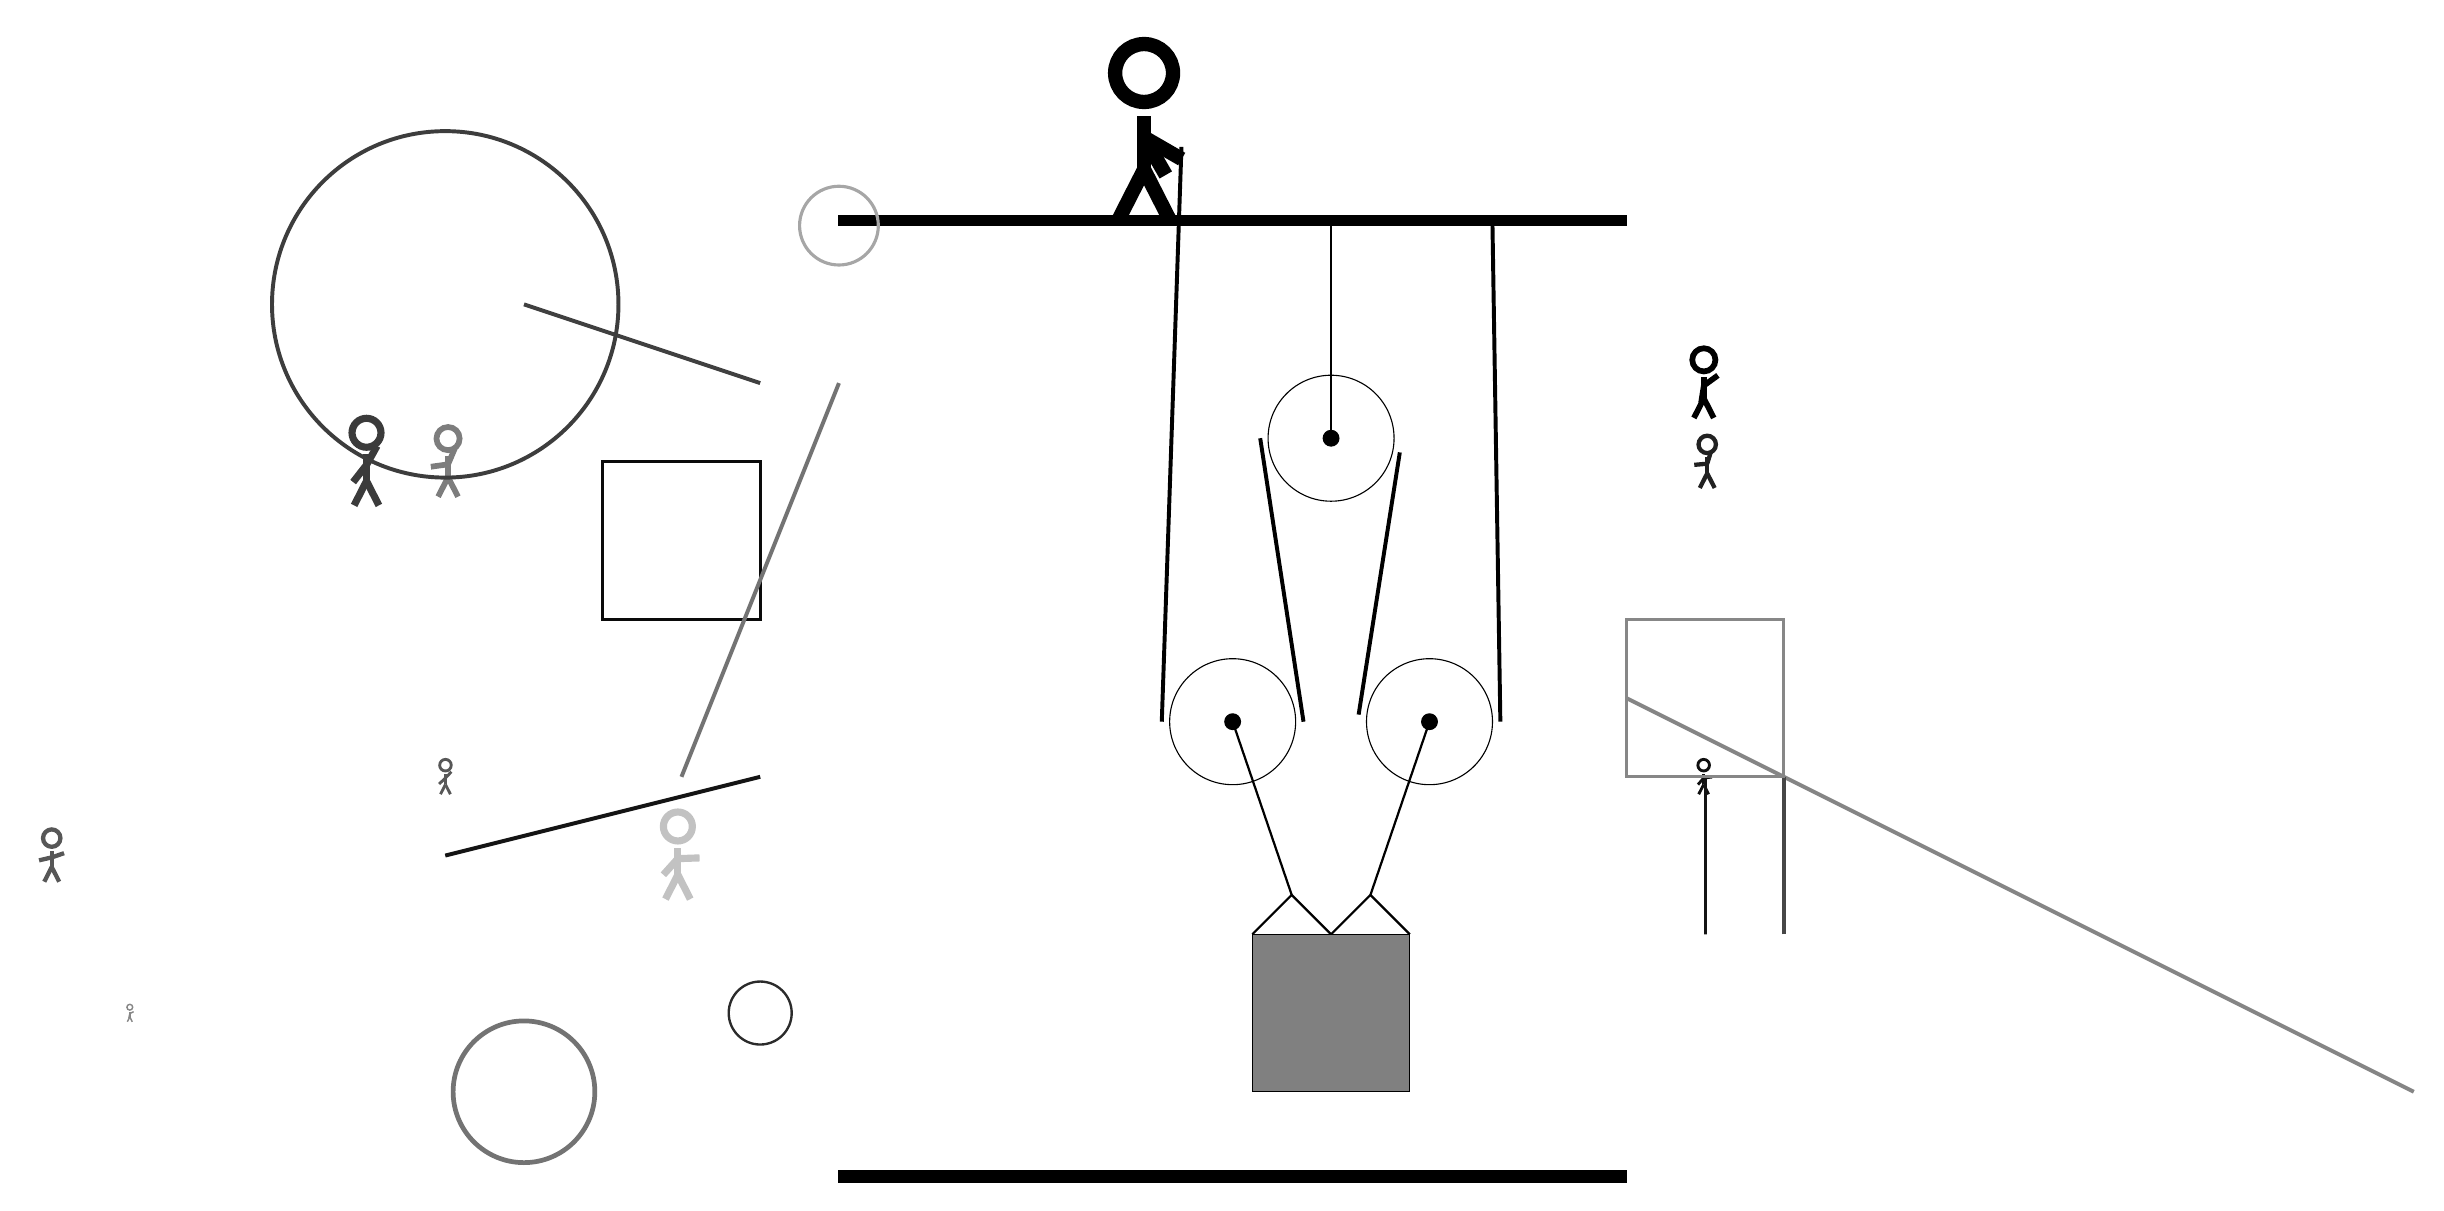
\begin{tikzpicture}
			%%%%% START %%%%%
			
			\draw[fill=black] (-4, 9) rectangle (6, 9.125);
			
			\draw (1, 2.7) circle (0.8);
			\draw[fill=black] (1, 2.7) circle (0.1);
			
			\draw (2.25, 6.3) circle (0.8);
			\draw[fill=black] (2.25, 6.3) circle (0.1);
			\draw[thick] (2.25, 6.3) -- (2.25, 9);
			
			\draw (3.5, 2.7) circle (0.8);
			\draw[fill=black] (3.5, 2.7) circle (0.1);
			
			\draw[thick] (3.5, 2.7) -- (2.75, 0.5);
			\draw[thick] (1, 2.7) -- (1.75, 0.5);
			\draw[thick]  (1.25, 0) -- (1.75, 0.5) -- (2.25, 0);
			\draw[thick]  (2.25, 0) -- (2.75, 0.5) -- (3.25, 0);
			\draw[fill=black!50] (1.25, 0) rectangle (3.25, -2);
			
			\draw[line width=0.5mm] (0.35, 10) --  (0.1, 2.7);
			\centerarc[line width=0.5mm](1, 2.7)(180:360:0.9);
			\draw[line width=0.5mm] (1.9, 2.7) -- (1.35, 6.3);
			\centerarc[line width=0.5mm](2.25, 6.3)(-20:180:0.9);
			\draw[line width=0.5mm](3.123, 6.12) -- (2.6, 2.79);
			\centerarc[line width=0.5mm](3.5, 2.7)(160:360:0.9);
			\draw[line width=0.5mm](4.4, 2.7) -- (4.3, 9);
			
			\node[line width=0.4mm, color=black!77] at (-10, 6) {\Strichmaxerl[5][52][61]};
			
			\draw[line width=0.5mm, color=black!92](-9, 1) -- (-5, 2);
			\draw [line width=0.3mm, color=black!83](-5, -1) circle (0.4);
			\draw[line width=0.4mm, color=black!96] (-5, 6) rectangle (-7, 4);
			\node[line width=0.5mm, color=black!66] at (-9, 2) {\Strichmaxerl[2][43][47]};
			\draw[line width=0.5mm, color=black!48](6, 3) -- (16, -2);
			
			\node[line width=0.2mm, color=black!94] at (7, 2) {\Strichmaxerl[2][49][7]};
			\node[line width=0.6mm, color=black!51] at (-9, 6) {\Strichmaxerl[4][8][67]};
			\draw[line width=0.5mm, color=black!75](-5, 7) -- (-8, 8);
			
			\node[line width=0.6mm, color=black!87] at (7, 6) {\Strichmaxerl[3][5][73]};
			\node[line width=0.6mm, color=black!100] at (7, 7) {\Strichmaxerl[4][81][36]};
			\draw[line width=0.5mm, color=black!55](-4, 7) -- (-6, 2);
			\draw[line width=0.5mm, color=black!72](8, 0) -- (8, 2);
			\draw [line width=0.6mm, color=black!55](-8, -2) circle (0.9);
			\draw[line width=0.4mm, color=black!92] (7, 2) rectangle (7, 0);
			\draw [line width=0.5mm, color=black!76](-9, 8) circle (2.2);
			
			\node[line width=0.7mm, color=black!66] at (-14, 1) {\Strichmaxerl[3][13][19]};
			\draw[line width=0.4mm, color=black!47] (8, 4) rectangle (6, 2);
			\node[line width=0.2mm, color=black!47] at (-13, -1) {\Strichmaxerl[1][78][27]};
			
			\draw [line width=0.4mm, color=black!35](-4, 9) circle (0.5);
			\node[line width=0.6mm, color=black!24] at (-6, 1) {\Strichmaxerl[5][48][2]};
			
			\node at (-0.07, 10.2) {\Strichmaxerl[10][120][-30]};
			
			\draw[fill=black] (-4, -3) rectangle (6, -3.15);
			
			%%%%% END %%%%%
		\end{tikzpicture}
	\end{figure}	
\end{document}